\documentclass{article}
\usepackage[utf8]{inputenc}
\usepackage{hyperref}
\usepackage{geometry}
 \geometry{
 a4paper,
 total={170mm,257mm},
 left=20mm,
 top=20mm,
 }
\linespread{1.2}

\title{Operator Product Expansion}
\author{Luigi Del Debbio, Joseph Lee, Andrew Yong}
\date{January 2019}

\usepackage{natbib}
\usepackage{graphicx}
\usepackage{amsmath}
\usepackage{amssymb}
\usepackage{textcomp}
\usepackage{empheq}
\usepackage{physics}
\usepackage{tikz-feynman}
\usepackage{float}
\usepackage{pifont}
\setcitestyle{square}

\begin{document}

\maketitle
\renewcommand{\abstractname}{\vspace{-\baselineskip}}
\begin{abstract}
These notes aim to supplement Collins' discussion on Operator Product Expansion (Ch.10, Renormalisation \cite{collins_1984}). Here we demonstrate how to obtain the Wilson coefficients in the (simple) case of $\phi^4$ theory. Useful references include \cite{schwartz}, \cite{Peskin:1995ev}, \cite{Bonneau:2009}. Figures in this document are either original or recreation of plots found in \cite{collins_1984} and \cite{weinberg}.
\end{abstract}

\section{Preamble}
First, a motivation. There are many cases when we are interested in computing the products of some operators, especially in the short distance limit. As an example, consider the high energy limit of the total hadronic $e^+ e^-$ cross section \cite{Bonneau:2009}
\begin{equation}
    \sigma_{e^+ e^-} \sim \int d^4x e^{iq\cdot x} \ev{T[J_\mu(x)J_\nu(0)]}{0}
\end{equation}
where $J_\mu$ is the electromagnetic hadronic current. A very significant contribution comes from the short distance expression of the vacuum polarisation matrix element 
\begin{equation}
    \lim_{x\rightarrow0} \ev{T[J_\mu(x)J_\nu(0)]}{0}
\end{equation}
We need some way to express the short distance behaviour of this product of operators, and this is where Operator Product Expansion (OPE) comes in. OPE refers to the expansion of a product of operators into a sum over local, composite, renormalised field operators. The difficulty in the procedure comes from the fact that the products become singular when their space-time points coincide; therefore we need a methodical procedure to identify the singular behaviour coming from the coinciding of space-time points (while separately taking care of divergences coming from loops in other parts of the diagram), then showing that they could form an expansion in terms of local (renormalised) operators with the singular functions as coefficients. The main objective of Collins' and our discussion here is to make precise what this means, justify that this procedure is possible and how exactly to perform it.



The objects we wish to study are the time-ordered products, e.g. $T\phi(x)\phi(0)$ and their Fourier transforms, defined as

\begin{equation}
    T\Tilde{\phi}(q)\phi(0) = \int d^4x e^{iq\cdot x} T\phi(x)\phi(0),
\end{equation}
where `T' as usual is the time-ordering operator. (Here and throughout the document we take $D=4$; the technique easily generalises)

We are interested in two highly related questions regarding these objects:

\begin{enumerate}
    \item \textbf{small-x limit}: What is the behaviour of $T\phi(x)\phi(0)$ when $x\rightarrow 0$? 
    \item \textbf{large-q limit}: What is the behaviour of $T\Tilde{\phi}(q)\phi(0)$ when $\vert q\vert \rightarrow\infty$?
\end{enumerate}

Thanks to efforts made by Wilson \cite{wilson} and company, we have a strategy to tackle these problems. Regarding the small-$x$ limit, the possibility of OPE tells us that we can express 
 \begin{equation}
     \lim_{x\rightarrow 0}T\phi(x)\phi(0) \sim \sum_\mathcal{O} C_\mathcal{O}(x)[\mathcal{O}(0)],
     \label{small x ope}
 \end{equation}
 where $[\mathcal{O}]$ are local renormalised operators and the coefficients $C_\mathcal{O}(x)$ are just c-numbers.  This is the general form of an OPE and the $C_\mathcal{O}$ are called the \textit{Wilson coefficients}. We of course expect in this case $\phi(x)\phi(0)$ (in leading order) to behave like a singular function of $x$, coupled with the renormalised $\phi^2$ operator, and in much of the remaining discussion we will focus on finding what $C_{\phi^2}(x)$ is.

 
 As for the large-$q$ behaviour, we start by considering the following momentum space Green's function:
 \begin{equation}
     \Tilde{G}_{N+2} = \mel{0}{T\Tilde{\phi}(q)\phi(0)\Tilde{\phi}(p_1)\dots\Tilde{\phi}(p_N)}{0},
 \end{equation}
 where $p_i,\forall i$ are fixed and we send $q\rightarrow \infty$. We claim there is an equivalent OPE of the form
 
 \begin{equation}
     \Tilde{G}_{N+2} \sim \sum_\mathcal{O} \Tilde{C}_\mathcal{O}(q) \mel{0}{T\mathcal{O}(0)\Tilde{\phi}(p_1)\dots\Tilde{\phi}(p_N)}{0}.
     \label{large q ope}
 \end{equation}
 Recall that $\Tilde{G}_{N+2}$ is the Fourier transform from coordinate to momentum space, that is
 
 \begin{equation}
     G_{N+2} \equiv \mel{0}{T\phi(x)\phi(0)\Tilde{\phi}(p_1)\dots\Tilde{\phi}(p_N)}{0} = \int \frac{d^4q}{(2\pi)^4} e^{-iq\cdot x}\Tilde{G}_{N+2}.
     \label{x-q fourier transform}
 \end{equation}
 With naive power counting, we see that if $\Tilde{G}_{N+2}$ falls as $1/q^4$ or slower for $q\rightarrow\infty$, then the LHS becomes a singular function of $x$, which is what we expect from the small-$x$ behaviour in Equation \ref{small x ope}. Thus, studying the large $q$ behaviour in Equation \ref{x-q fourier transform} aids us in understanding the singular $x\rightarrow 0$ limit in coordinate space. 
 
 In the following, we will begin by examining the small-$x$/large-$q$ behaviours in the $\phi^4$ theory. We restrict ourselves to studying Green's functions of $\phi(x)\phi(0)$. We will look at how to obtain the Wilson Coefficient to $\mathcal{O}(1)$ in section \S\ref{10.1.1} and $\mathcal{O}(g)$ in \S\ref{10.1.2}, where we will first encounter the effects coming from small x. We will then review Weinberg's theorem in section \S\ref{prerequesites} which will prepare us to understand the recipe for obtaining the Wilson coefficients  in section \S\ref{proof} as laid out by Collins, and finally conclude with applying the procedure to 1 of 2 diagrams which contribute to the Wilson coefficient to $\mathcal{O}(g^2)$.
%  Comparing Equation \ref{small x ope}, \ref{large q ope}and \ref{x-q fourier transform}, we find that the large-$q$ behaviour is dominated by singularities in $x$-space. Since the singularities in $x$-space occurs as $x\rightarrow 0$, 
 
 
\section{Non-Divergent Example}\label{10.1.1}

Let us begin with a non-divergent example. Consider the usual $\phi^4$ theory:

\begin{equation}
    \mathcal{L} = \frac{1}{2}\partial^\mu\phi\partial_\mu\phi - \frac{1}{2}m^2\phi^2 - \frac{g}{4!}\phi^4.
\end{equation}
We want to study Green's functions of the form $\phi(x)\phi(0)$, so let us consider the time-ordered correlation function of the form

\begin{equation}
    \mel{0}{T\phi(x)\phi(0)\Tilde{\phi}(p_1)\Tilde{\phi}(p_2)}{0},
    \label{time ordered}
\end{equation}
where the `$T$' is the usual time-ordering and $\Tilde{\phi}(p)$ are field operators projected to a specific 4-momentum, $p$. This is illustrated in Figure \ref{fig:10.1.1}.

\begin{figure}[H]
\centering
\includegraphics*[width=0.5\textwidth]{Graphs/Fig1011a.eps}
\caption{Possible $\mathcal{O}(1)$ graphs. }
\label{fig:10.1.1}
\end{figure}\\

Note that Equation \ref{time ordered} is the $\mathcal{O}(1)$ term in our $\phi^4$ theory. To evaluate it, we simply perform a Fourier transform on the $\Tilde{\phi}$ and then apply Wick's theorem:

\begin{equation}
    \begin{split}
        \mel{0}{T\phi(x)\phi(0)\Tilde{\phi}(p_1)\Tilde{\phi}(p_2)}{0}&=\int d^4x_1d^4x_2 e^{-ip_1\cdot x_1}e^{-ip_2\cdot x_2}\mel{0}{T\phi(x)\phi(0)\phi(x_1)\phi(x_2)}{0},\\
        &=\int d^4x_1d^4x_2 e^{-ip_1\cdot x_1}e^{-ip_2\cdot x_2}\mel{0}{(\overbrace{\phi(x)\phi(x_1)}\overbrace{\phi(0)\phi(x_2)} + x_1\leftrightarrow x_2 + \dots)}{0},\\
        &= \int \frac{d^4x_1d^4x_2d^4k_1d^4k_2}{(2\pi)^8} e^{ip_1\cdot x_1}e^{ip_2\cdot x_2} \left(\frac{ie^{-ik_1\cdot (x-x_1)}}{k_1^2-m^2}\frac{ie^{-ik_2\cdot x_2}}{k_2^2-m^2}+ x_1\leftrightarrow x_2 \right),\\
        &= \int_{x_1,x_2,k_1,k_2}  \left(\frac{ie^{-ix_1\cdot (k_1-p_1)}e^{-ik_1\cdot x}}{k_1^2-m^2}\frac{ie^{-ix_2\cdot (k_2-p_2)}}{k_2^2-m^2}+ x_1\leftrightarrow x_2 + \dots\right),\\
        &= \int_{k_1,k_2}  \left(\frac{i\delta^3(k_1-p_1)e^{-ik_1\cdot x}}{k_1^2-m^2}\frac{i\delta^3(k_2-p_2)}{k_2^2-m^2}+ x_1\leftrightarrow x_2 \right),\\
        \mel{0}{T\phi(x)\phi(0)\Tilde{\phi}(p_1)\Tilde{\phi}(p_2)}{0}&= \frac{i}{p_1^2-m^2}\frac{i}{p_2^2-m^2}(e^{-ip_1\cdot x}+e^{-ip_2\cdot x}),\\
    \end{split}
\end{equation}
where the $\dots$ represent any normal-ordered products (which annihilates the vacuum) and any disconnected diagrams(\textit{e.g} $\overbrace{\phi(x)\phi(0)}$ ).

If we perform a power expansion on $x$, one finds

\begin{equation}
    \frac{i}{k_1^2-m^2}\frac{i}{k_2^2-m^2}(e^{-ip_1\cdot x}+e^{-ip_2\cdot x})=\frac{i}{k_1^2-m^2}\frac{i}{k_2^2-m^2}(2-i(p_1+p_2)\cdot x -\frac{1}{2!}\left( (p_1\cdot x)^2 + (p_2\cdot x)^2\right) + \dots ).
    \label{small x expansion}
\end{equation}
Thus, if we examine the matrix element carefully, we find that this expansion is equivalent to the replacement

\begin{equation}
    T\phi(x)\phi(0) = \phi^2(0) + \frac{1}{2}
x^\mu\partial_\mu\phi^2 + \frac{1}{2} x^\mu x^\nu\phi\partial_\mu\partial_\nu\phi + \dots,
\label{taylor expansion}
\end{equation}
when we send $x\rightarrow 0$.

Comparing with Equation \ref{small x ope}, we see that for the free-field theory (no interactions), the OPE is just a Taylor expansion of $\phi(x)$ about $x=0$. Since we must preserve the dimension of the operators on LHS and RHS, the Wilson coefficients in this case should take the following form:

\begin{equation}
    C_\mathcal{O}(x) = \mathrm{const.}\,\times\vert x\vert^a,
\end{equation}
where $a=\mathrm{dim}[\mathcal{O}]-\mathrm{dim}\,[\phi(x)\phi(0)]$. To see that this is true, consider the second term in Equation \ref{taylor expansion}. The operator is now $\mathcal{O}=\partial_\mu\phi^2$ with $\mathrm{dim}[\mathcal{O}]=-1+(-2)=-3$ in length dimensions. Thus, it is clear that $a=1$ is required to match the length dimensions.

Another non-trivial divergence-free example is the `four-point correlator' at $\mathcal{O}(g^2)$. It has the form shown in Figure \ref{fig:10.1.2}.

\begin{figure}[H]
\centering
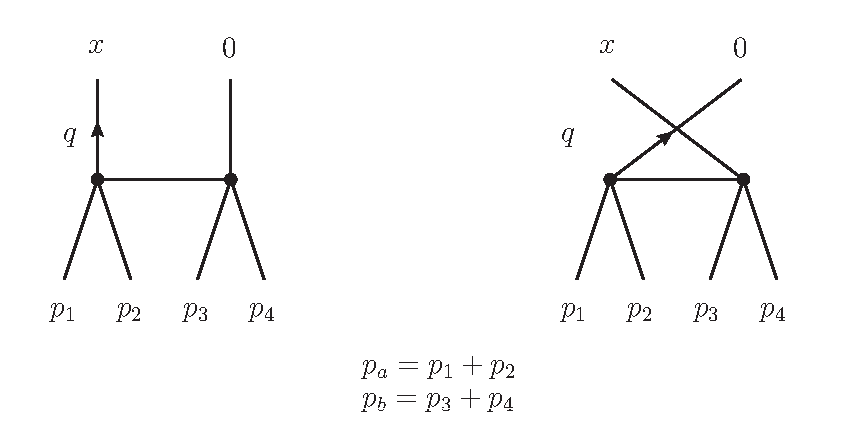
\includegraphics[width=0.5\textwidth]{Graphs/Fig1012.eps}
\caption{Possible $\mathcal{O}(g^2)$ graphs. Here, $q$ is an undetermined momentum.}
\label{fig:10.1.2}
\end{figure}\\

Computing the four-point function is similar to the two-point function we illustrated above, so we leave that as an exercise to the reader. The important factor from this four-point function comes from the line with momentum $q$:

\begin{equation}
    \mel{0}{T\phi(x)\phi(0)\Tilde{\phi}(q)\Tilde{\phi}(p_1)\dots\Tilde{\phi}(p_4)}{0} \sim ig^2\int \frac{d^4q}{(2\pi)^4}\frac{e^{-iq\cdot x}+e^{i(q-p_a-p_b)\cdot x}}{(q^2-m^2)[(p_a-q)^2-m^2][(q-p_a-p_b)^2-m^2]}
\end{equation}

Now, if we expand in powers of small $x$ as before, we find 

\begin{equation}
    \begin{split}
        \mel{0}{T\phi(x)\phi(0)\Tilde{\phi}(q)\Tilde{\phi}(p_1)\dots\Tilde{\phi}(p_4)}{0} &\sim ig^2\int \frac{d^4q}{(2\pi)^4}\frac{1-iq\cdot x -\frac{1}{2}(q\cdot x)^2+\dots}{(q^2-m^2)[(p_a-q)^2-m^2][(q-p_a-p_b)^2-m^2]}\\
        &+ \frac{1+i(q-p_a-p_b)\cdot x+ -\frac{1}{2!}((q-p_a-p_b)\cdot x)^2+\dots}{(q^2-m^2)[(p_a-q)^2-m^2][(q-p_a-p_b)^2-m^2]},\\
        &\sim ig^2\int \frac{d^4q}{(2\pi)^4}\frac{2 - i(p_a+p_b)\cdot x +\dots}{(q^2-m^2)[(p_a-q)^2-m^2][(q-p_a-p_b)^2-m^2]},
    \end{split}
\end{equation}
where the $\dots$ indicate terms with higher powers of $q$. We identify these first two terms as in Equation \ref{small x expansion}. However, when we consider $\mathcal{O}(q^n)$ terms with $n\geq 2$, the integral becomes ultraviolet divergent.  We will deal with these divergences in the following section. For convenience, we will restrict our attention to the leading power behaviour. This will correspond to the $\phi^2$ term in Equation \ref{taylor expansion}. 

\section{Divergent Example}\label{10.1.2}
In \S\ref{10.1.1}, we have been exploring the tree-level expansion of the two point function $T\phi(x)\phi(0)$. As explained at the end of \S\ref{10.1.1}, we will be restricting our attention to the leading-power behaviour, i.e. studying
\begin{align}
\label{c_phi2}
    T\phi(x)\phi(0) \sim C_{\phi^2}(x)[\phi^2]
\end{align}
where $[\phi^2]$ is the renormalised Green's function. \\

In this `divergent example', we evaluate the correction to $T\phi(x)\phi(0)$. At order $\mathcal{O}(g)$, the correction is given by
\begin{equation}
    \frac{i^2}{(p_1^2-m^2)(p_2^2-m^2)}ig\int \frac{d^4q}{(2\pi)^4} \frac{e^{-iq\cdot x}}{(q^2-m^2)((q-p_1-p_2)^2 - m^2)}.
    \label{loopOg}
\end{equation}
which corresponds to the Feynman diagram in Figure \ref{fig:10.1.3abc}(a).\\

\begin{figure}[H]
\centering
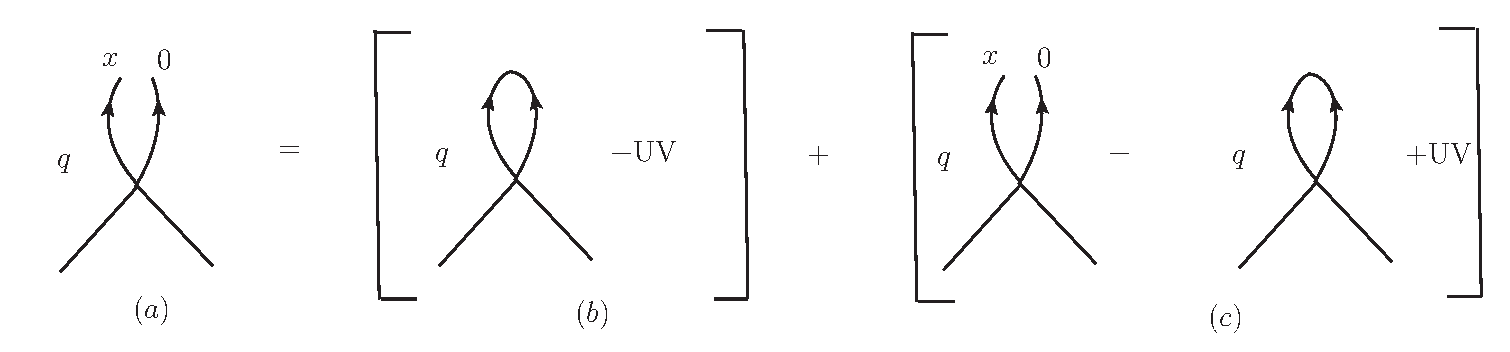
\includegraphics[width=0.75\textwidth]{Graphs/Fig1013abc.eps}
\caption{Regulating the $\mathcal{O}(g^2)$ graphs.}
\label{fig:10.1.3abc}
\end{figure}\\

Two regions of momentum $q$ contribute differently to this term:
\begin{enumerate}
    \item $q$ finite as $x \rightarrow 0$, this  provides an $x-$independent correction,
    \item $q$ large (up to $O(1/x)$) as $x \rightarrow 0$, this  provides an $x-$dependent correction.
\end{enumerate}
As we will see, this allows us to express 
\begin{align}
    C_{\phi^2} = 1 + (g/16\pi^2)c_1(x^2)
\end{align}
for some $c_1$ which we will calculate. The two momentum regions contribute to the two terms respectively, and they correspond to the decomposition of Figure \ref{fig:10.1.3abc}(a) into (b) and (c), where (b) is simply performing renormalisation to $\phi(0)^2$ by cutting off the UV divergence, and (c) takes care of the remaining contribution. 
\subsection{Momentum Region 1: $q$ finite, $x\rightarrow 0$}

In the region where $q$ is finite, sending $x\rightarrow 0$ (so $e^{-iq\cdot x} \rightarrow 1$) will get  us the standard logarithmic divergent term of the form 

\begin{equation}
    \frac{i^2}{(p_1^2-m^2)(p_2^2-m^2)}ig\int \frac{d^4q}{(2\pi)^4} \frac{1}{(q^2-m^2)((q-p_1-p_2)^2 - m^2)}.
    \label{logdiv}
\end{equation}

Let us be very explicit here. To renormalise this, we can use dimensional regularisation to expose the divergent terms. First, we apply the Feynman parameter trick to Equation \ref{logdiv},

\begin{equation}
    \frac{1}{AB} = \int_0^1 dx \, \frac{1}{(A(1-x) + Bx)^2}.
\label{Feynparam trick}
\end{equation}
Identifying $A=(q^2-m^2)$ and $B=((q-p)^2-m^2)$, with $p=p_1+p_2$, the integral in Equation \ref{logdiv} becomes

\begin{equation}
\begin{split}
    I(p) &= ig\int \frac{d^4q}{(2\pi)^4}\int^1_0 dx \frac{1}{((q^2-m^2)(1-x) +(q-p_1-p_2)^2 - m^2)x)^2},\\
    &= ig\int \frac{d^4q}{(2\pi)^4}\int^1_0 dx \frac{1}{((q-px)^2 + p^2x(1-x) - m^2 )^2},\\
    \mathrm{let}\, q'&= q-px,\\
    &= ig\int \frac{d^4q}{(2\pi)^4}\int^1_0 dx \frac{1}{(q^2 -M^2)},
    \label{b4dimreg}
\end{split}
\end{equation}
where $M^2=M^2(s,x)=m^2-sx(1-x)$ and $s$ is the centre-of-mass energy, $s=p^2$. In the following, we will suppress the arguments of $M$ for brevity.

Next, we can Wick rotate to Euclidean momenta and generalise this integral to $D$-dimensions. This is captured by the following identity, 
\begin{equation}
    \int\frac{d^Dq}{(2\pi)^D} \frac{q^{2a}}{(q^2-M^2)^b}=\frac{i}{(4\pi)^{D/2}}\frac{(-1)^{a-b}}{(M^2)^{b-a-D/2}} \frac{\Gamma(a+\frac{D}{2})\Gamma(b-a-\frac{D}{2})}{\Gamma(b)\Gamma(\frac{D}{2})}
\end{equation}
which one can find in standard textbooks like \cite{schwartz}. Here, $\Gamma(x)$ is the gamma function, where $\Gamma(x) = (x-1)! = (x-1)\Gamma(x-1)$, with $\Gamma(1)=1$. Moreover, for $D\neq 4$, the coupling $g$ for a $\phi^4$ theory will be dimensionful. We can keep $g$ dimensionless by performing the replacement
\begin{equation}
    g \rightarrow \mu^{4-D}g.
\end{equation}
Identifying $a=0$ and $b=2$ in Equation \ref{b4dimreg}, we have 

\begin{equation}
    \begin{split}
        I(p) &= ig\mu^{4-D} \frac{i}{(4\pi)^{D/2}}\frac{\Gamma(\frac{D}{2})\Gamma(2-\frac{D}{2})}{\Gamma(2)\Gamma(\frac{D}{2})}\int^1_0 dx \, \frac{(-1)^{-2}}{(M^2)^{2-D/2}},\\
        &= ig\mu^{4-D} \frac{i}{(4\pi)^{D/2}}\Gamma(2-\frac{D}{2})\int^1_0 dx \, \frac{1}{(M^2)^{2-D/2}},\\
    \end{split}
\end{equation}

Now, we let $D=4-2\epsilon$. Then, $I(p)$ becomes

\begin{equation}
    I(p)=ig\frac{i}{16\pi^2}(4\pi)^{\epsilon}\Gamma(\epsilon)\int^1_0 dx \, \left(\frac{\mu^2}{M^2}\right)^{\epsilon},
\end{equation}

Recall that, in the limit of $\epsilon\rightarrow 0$, we can make the following approximation:

\begin{equation}
\begin{split}
    u^\epsilon &= 1 + \epsilon \log{u} + \mathcal{O}(\epsilon),\\
    \Gamma(\epsilon) &= \frac{1}{\epsilon} - \gamma_E + \mathcal{O}(\epsilon),
\end{split}
\end{equation}
where $u$ is some polynomial of order $\epsilon$ and $\gamma_E$ is the Euler-Mascheroni constant.

Using the relations above, $I(p)$ becomes

\begin{equation}
    \begin{split}
       I(p)&=ig\frac{i}{16\pi^2}\int^1_0 dx \, (1+\epsilon\log{4\pi} + \mathcal{O}(\epsilon))(\frac{1}{\epsilon} - \gamma_E + \mathcal{O}(\epsilon))(1+\epsilon\log{\frac{\mu^2}{M^2}}+ \mathcal{O}(\epsilon)),\\
       &=ig\frac{i}{16\pi^2}\int^1_0 dx \, \frac{1}{\epsilon} - \gamma_E + \log{\frac{4\pi\mu^2}{M^2}} + \mathcal{O}(\epsilon).
    \end{split}
\end{equation}

Now, we apply the MS subtraction scheme, where the $\epsilon$ terms are removed from the integral. At last, Equation \ref{logdiv} becomes 

\begin{equation}
     \frac{i^2}{(p_1^2-m^2)(p_2^2-m^2)}\frac{-g}{16\pi^2}\int^1_0 dx \, \log{\frac{4\pi\mu^2}{M^2}} - \gamma_E.
\end{equation}
And this is the order 1 contribution to the correction from the first momentum region.

\subsection{Momentum Region 2: large $q \sim O(1/x)$}\label{large q}
The remaining contribution is in equation (10.1.13):
\begin{equation} \label{eq:div_eg_large_q}
    \frac{i^2}{(p_1^2-m^2)(p_2^2-m^2)}\frac{ig}{(2\pi)^4}\cross\qty{\int d^4q \frac{e^{iq\cdot x}-1}{(q^2-m^2)[(q-p_1-p^2)^2-m^2]}-\text{UV divergence}}
\end{equation}
For this term, the region where $q$ becomes large up to $O(1/x)$ as $x \rightarrow 0$ is important, since it provides a contribution of order 1 (as $q\cdot x \sim 1$). This is to be contrasted with the region of finite $q$, where the contribution is of order $\abs{x}$. We again note that, as will be shown, the UV divergence here is equal to that present in the first region(finite $q$), therefore the decomposition makes sense (and that this diagram is in fact finite and no renormalisation is required).

As we are considering large $q \sim 1/x$, we can see that $p_1$, $p_2$ (momenta in the lower legs) and $m$ does not provide leading-power contribution to the term in the curly-bracket (differentiating the term w.r.t $p_1$, $p_2$ or $m$ will always bring another power of $q$ to the denominator, lowering the order of the integral; in this case it results in a convergent finite integral, which goes to $0$ as some power of $x$ when $x \rightarrow 0$). We can therefore ignore these variables and set $m=p_1=p_2=0$ in defining $c_1(x)$. \\

Consider the term
\begin{equation}
\begin{split}
    &\ \text{i}\int d^4q\frac{e^{iq\cdot x}-1}{(q^2)^2} \\
    &\rightarrow\frac{\text{i}}{(2\pi\mu)^{D-4}}\int d^Dq\frac{e^{iq\cdot x}-1}{(q^2)^2} \text{ - analytically continue to dim D, with } g \rightarrow \mu^{4-D}g\\
    &= \frac{\text{ig}}{(2\pi\mu)^{D-4}}\int d^Dq \int_0^\infty  dz\ z e^{-z(-q^2)} (e^{iq\cdot x}-1) \text{ - using identity provided}\\
    &= \frac{-1g}{(2\pi\mu)^{D-4}}\int d^Dq \int_0^\infty  dz\ z e^{-z(q^2)} (e^{-iq\cdot x}-1) \text{ - wick rotation}\\
    &= \frac{-1}{(2\pi\mu)^{D-4}}\int d^Dq \int_0^\infty  dz\ z (e^{-z(q^2+iq\cdot x/z+(ix/2z)^2)-x^2/4z}-e^{-z(q^2)}) \text{ - complete the square}\\
    &= \frac{-1}{(2\pi\mu)^{D-4}}\int d^Dq \int_0^\infty  dz\ z (e^{-z(q+ix/2z)^2}e^{-x^2/4z}-e^{-z(q^2)})\\
    &= \frac{-1}{(2\pi\mu)^{D-4}}\int_0^\infty  dz\ z (\frac{\pi}{z})^{D/2}(e^{-x^2/4z}-1)\text{ - gaussian integral}\\
\end{split}
\end{equation}

substitute $t = \frac{x^2}{4z},\ dz=-\frac{x^2}{4t^2}dt,\ \int_0^\infty \rightarrow \int_\infty^0$
\begin{equation}
\begin{split}    
    &= \frac{-1}{(2\pi\mu)^{D-4}}\int_0^\infty  dt\ \frac{x^2}{4t^2} \frac{x^2}{4t}
    (\frac{4\pi t}{x^2})^{D/2}(e^{-t}-1)\\
    &= \frac{-\pi^{D/2}(x^2)^{2-D/2}}{(2\pi\mu)^{D-4}4^{2-D/2}}\int_0^\infty  dt\ t^{D/2-3}(e^{-t}-1)
\end{split}
\end{equation}
using $\Gamma(z)=\int_0^\infty dt\ t^{z-1}e^{-t}$
\begin{equation}
    = \frac{-\pi^{D/2}(x^2)^{2-D/2}}{(2\pi\mu)^{D-4}4^{2-D/2}}(\Gamma(\frac{D}{2}-2)-\eval{\frac{t^{D/2-2}}{D/2-2}}_0^\infty )
\end{equation}
using the property that $\int d^Dp(p^2)^\alpha = 0$ (see Collins, p.73 eq 4.3.1a), we see that the second term vanishes. Now, we set $D=4-2\epsilon$
\begin{equation}
\begin{split}
    &= \frac{-\pi^{2-\epsilon}(x^2)^{\epsilon}}{(2\pi\mu)^{-2\epsilon}2^{2\epsilon}}\Gamma(-\epsilon)\\
    &= -\pi^2(\pi\mu^2 x^2)^\epsilon\Gamma(-\epsilon)\\
    &= -\pi^2 (1+\epsilon \ln(\pi \mu^2 x^2)+O(\epsilon^2))(-\frac{1}{\epsilon}-\gamma_E+O(\epsilon))\\
    &= \pi^2(\frac{1}{\epsilon}+\gamma_E+\ln(\pi\mu^2 x^2)+O(\epsilon))\\
    i\int d^4q\frac{e^{iq\cdot x}-1}{(q^2)^2}&= \pi^2(\frac{1}{\epsilon}+\gamma_E+\ln(-\pi\mu^2 x^2)+O(\epsilon))\text{ - Wick rotate back}
\end{split}
\end{equation}

Therefore
\begin{equation}
    \frac{ig}{(2\pi)^4}\cross\qty{\int d^4q \frac{e^{iq\cdot x}-1}{(q^2-m^2)[(q-p_1-p^2)^2-m^2]}} = \frac{g}{16\pi^2}\qty{\frac{1}{\epsilon}+\gamma_E+\ln(-\pi\mu^2 x^2)}
\end{equation}
As we can see, this term has the same pole/UV-divergence as that from the first region, and so the decomposition makes sense. And now we can identify
\begin{equation}
\begin{split}
    c_1(x) &= \frac{1}{2\pi^2} \qty{\frac{\text{i}}{(2\pi\mu)^{D-4}}\int d^Dq\frac{e^{iq\cdot x}-1}{(q^2)^2}-\frac{2}{D-4}}\\
    &=\frac{1}{2\pi^2} \qty{\pi^2(\frac{1}{\epsilon}+\gamma_E+\ln(-\pi\mu^2 x^2)+O(\epsilon))-\frac{1}{\epsilon}}\\
    c_1(x)&=\frac{1}{2}(\gamma_E+\ln(-\pi\mu^2 x^2))
\end{split}
\end{equation}

\section{Some Pre-requisites} \label{prerequesites}
\subsection{Weinberg's Theorem}
In the divergent example, we have seen how to treat the contribution from the large $q$ region for the specific diagram. There we can easily see that the leading order $q$ contribution (Equation \ref{eq:div_eg_large_q}) has to come from the single loop, then can we argue from there that the leading power contribution from the loop does not depend on the external momenta/mass. In this case, identifying and isolating the large $q$ behaviour is easy. To be able to generalise the discussion to any diagrams, we have to understand the behaviour of a general graph when the internal momentum $q$ is large; this is where Weinberg's theorem \cite{weinberg} comes in. In essence, Weinberg's theorem allows us to identify and isolate/factorise the largest power contribution from a given diagram. Before we can discuss the theorem itself, we have to understand the concept of subgraphs.\\



\subsubsection{Subgraphs}
\textbf{Definition}: A set $\mathcal{G'}$ of internal and external lines $j$ form a subgraph of $\mathcal{G}$ provided that there is no vertex in $\mathcal{G}$ to which is attached just one line of those in $\mathcal{G'}$. In other words, a subgraph $\mathcal{G'}$ is composed of a number of paths which begin and end in external lines or each other, but never end abruptly within $\mathcal{G}$. 

\subsubsection{Example of Subgraphs}
For this diagram:
\begin{center}
    \feynmandiagram [small, horizontal=a to b] {
    i1 -- [plain] a -- [plain] c -- [plain] i3,
    i2 -- [plain] b -- [plain] d -- [plain] i4,
    a -- [photon] b,
    d -- [photon] c,   
    }
\end{center}
Subgraphs (in bold) include:\\
\begin{center}    
    \feynmandiagram [small, horizontal=a to b] {
    i1 -- [plain, very thick] a -- [plain, very thick] c -- [plain, very thick] i3,
    i2 -- [plain] b -- [plain] d -- [plain] i4,
    a -- [photon] b,
    d -- [photon] c,
    };
    \feynmandiagram [small, horizontal=a to b] {
    i1 -- [plain, very thick] a -- [plain] c -- [plain, very thick] i3,
    i2 -- [plain] b -- [plain, very thick] d -- [plain] i4,
    a -- [photon, very thick] b,
    d -- [photon, very thick] c,
    };
    \feynmandiagram [small, horizontal=a to b] {
    i1 -- [plain, very thick] a -- [very thick, plain] c -- [plain, very thick] i3,
    i2 -- [plain] b -- [plain, very thick] d -- [plain] i4,
    a -- [photon, very thick] b,
    d -- [photon, very thick] c,
    };...\\
\end{center}

\subsubsection{Theorem}
Consider a Feynman diagram $\mathcal{G}$ in any local field theory. Any external or internal lines $j$ in this diagram is associated with a bare propagator $\Delta_j(p_j,\sigma)$, where $p_j$ is the four-momentum carried by the line $j$, and $\sigma$ is the label that contains all discrete variables such as spins, polarizations, etc. The integrand $F$ corresponding to the diagram $\mathcal{G}$  is given as the product
\begin{equation}
    F= \gamma(\sigma)\prod_{j=1}^M \Delta_j(p_j,\sigma)
\end{equation}
over all lines $M$. $\gamma(\sigma)$ here is the product of all vertex factors including Dirac matrices, coupling constants etc. \\

The Green's function corresponding to $\mathcal{G}$ is given by the integrating $F$ over the internal momenta:

\begin{equation}
    G(\mathbf{P}\in E, \sigma_{ext}) = \sum_{\sigma_{int}}\int_{\mathbf{P'}\in I}F(\mathbf{P+P'},\sigma) d\mathbf{P'}
\end{equation}
Here $E/I$ denotes the subspace of external/internal momenta. (Here we join the vector spaces of the external momenta and internal momenta into one big vector space)\\

The theorem tells us that for the integral $G$ (with Wick-rotated contour):
\begin{enumerate}
    \item $G$ converges if 
    \begin{enumerate}
        \item it converges superficially (i.e. $D_I:=\alpha(I)+\text{dim}I<0$) and 
        \item all sub-integrations converge superficially (i.e. $D_{I'}=\alpha(I')+\text{dim}I'<0$ for $I'\subset I$)
    \end{enumerate}
\end{enumerate}
Here $D_I$ is the \textit{superficial degree of divergence} of the integral, and the \textit{asymptotic coefficient} $\alpha(S)$ is defined by $F(\mathbf{L}\eta+\mathbf{C}) = O(\eta^{\alpha(\mathbf{L})})$ for $\mathbf{L}\in S$, i.e. the power scaling with a momentum vector in $V$. (for complete definition, see \cite[\S III]{weinberg})

\begin{enumerate}
\setcounter{enumi}{1}
    \item For any $S \subset E$, the asymptotic coefficient of $G$: $\alpha_I(S)=\max\limits_{\mathcal{G'}\ni S} \mathcal{D}_I(\mathcal{G'})$, where the max here is over all subgraphs $\mathcal{G'}$ which contains just the set $\mathcal{E}_\infty$ of external lines $j$ for which $\mathbf{V}_j$ is not orthogonal to $S$ (this condition is true for `almost any' choice of $p_j$, detail see \cite[\S V]{weinberg}). 
\end{enumerate}
Here $\mathcal{D}_I$ is called the \textit{dimensionality}, and it is the net number of momentum factors of the subgraph $\mathcal{G'}$, counting the momentum power $\alpha_j$ for each line $j$ ($-2$ for boson and $-1$ for fermion) and 4 for each integration. 

In other words, the second part of the theorem tells us that for a graph $\mathcal{G}$, if we let the momentum of a set of external lines $\mathcal{E}_\infty$ go to infinity, then the integrated Green's function corresponding to $\mathcal{G}$ will behave as $O\{\eta^{\alpha_I(\mathcal{E}_\infty)}(\log \eta)^{\beta_I(\mathcal{E}_\infty)}\}$, where $\alpha_I(\mathcal{E}_\infty)$ is the maximum of the dimensionality of all subgraphs $\mathcal{G'}$ of $\mathcal{G}$ including the external lines $\mathcal{E}_\infty$ and no other external lines.

\subsubsection{Example}
Let us try to figure out the behaviour of this graph as $k \rightarrow \infty$:\\
\begin{center}
    \feynmandiagram [small, horizontal=a to b] {
    i1 -- [fermion, edge label=\(k\)] a -- [fermion, edge label=\(k+p-q\)] c -- [fermion, edge label=\(k+p-p'\)] i3,
    i2 -- [fermion, edge label'=\(p\)] b -- [fermion, edge label'=\(q\)] d -- [fermion, edge label'=\(p'\)] i4,
    a -- [photon, edge label'=\(q-p\)] b,
    d -- [photon, edge label'=\(q-p'\)] c,
}
\end{center}

The corresponding integral (excluding external legs) is roughly (ignoring vertex and gamma factors/slashes etc.):
\begin{equation}
\begin{split}    
    \int \frac{d^4q}{(2\pi)^4}\frac{k+p-q}{(k+p-q)^2+m^2}\frac{k+p-p'}{(k+p-p')^2+m^2}\frac{1}{(q-p')^2+\mu^2}\frac{1}{(q-p)^2+\mu^2}\frac{q}{q^2+m^2}
\end{split}
\label{example graph integral}
\end{equation}
Part 2 of the theorem tells us to look at all subgraphs with the two external legs containing $k$, i.e. the two external legs on the left hand side, and no other external legs. This gives us the three subgraphs we presented before:\\
\begin{center}
    a:
    \feynmandiagram [small, horizontal=a to b] {
    i1 -- [fermion, very thick] a -- [fermion, very thick] c -- [fermion, very thick] i3,
    i2 -- [fermion] b -- [fermion] d -- [fermion] i4,
    a -- [photon] b,
    d -- [photon] c,
    };
    b:
    \feynmandiagram [small, horizontal=a to b] {
    i1 -- [fermion, very thick] a -- [fermion] c -- [fermion,  very thick] i3,
    i2 -- [plfermionain] b -- [fermion, very thick] d -- [fermion] i4,
    a -- [photon, very thick] b,
    d -- [photon, very thick] c,
    };
    c:
    \feynmandiagram [small, horizontal=a to b] {
    i1 -- [fermion, very thick] a -- [very thick, fermion] c -- [fermion, very thick] i3,
    i2 -- [fermion] b -- [fermion, very thick] d -- [fermion] i4,
    a -- [photon, very thick] b,
    d -- [photon, very thick] c,
}\\
\end{center}
The dimensionality of each graph could be calculated by summing $-2$ for each internal boson line, $-1$ for each internal fermion line and $4$ for each loop:
\begin{equation}
\begin{split}
    &\mathcal{D}_a= -1,\\ &\mathcal{D}_b= -2-1-2=-5,\\ &\mathcal{D}_c= -1-1-2-2+4=-2,  
\end{split}
\end{equation}
The maximum is $\mathcal{D}_a= -1$, therefore as $k \rightarrow \infty$, the integral goes as $k^{-1}$ (times some log). Note that this result is different from what we would naively expect from power counting in Equation \ref{example graph integral}. There, in the large $k$ regime, we would expect the integrand to scale as $\sim k^{-2}$. This highlights the importance of identifying divergent subgraphs in Weinberg's theorem. 

\subsection{Strategy of Proof}
\subsubsection{Large $q$ Subgraphs: $U$}
Weinberg's theorem tells us that to identify the leading power behaviour of a diagram when the momentum $q$ is large, we have to look at the subgraph with the largest power of momentum. In the case of our OPE expansion (in momentum space), we have to consider those subgraphs which contains $\phi(q)$ and $\phi(0)$ as external legs. 

For our scalar $\phi^4$ theory, we can show that subgraphs with the greatest power of momentum must only have 2 extra external legs other than $\phi(0)$ and $\phi(q)$. We can see this by using the usual divergence counting method:
\begin{equation}
\begin{split}
    &D=4L-2P,\\
    &L=P-V,\\
    &V=\frac{1}{4}(2P+E),\\
    &\Rightarrow D=-E.
\end{split}
\end{equation}
where $D$ is the degree of divergence, $L$ the number of loops, $P$ the number of propagators, $E$ number of external legs and $V$ number of vertices. We therefore want the subdiagram with as few external lines as possible; in our case, it will be 4, i.e. 2 extra external legs (on top of the $\phi(x)$ and $\phi(0)$ legs). 

Because of this, the subgraphs contributing to the leading power $q$ will take the form of the subgraph U in Figure \ref{fig:10.2.1}, in which all lines carry momentum of order $q$, with two lines with momenta $k$ and $l$ connecting to the IR subgraph I. 

\begin{figure}[H]
\centering
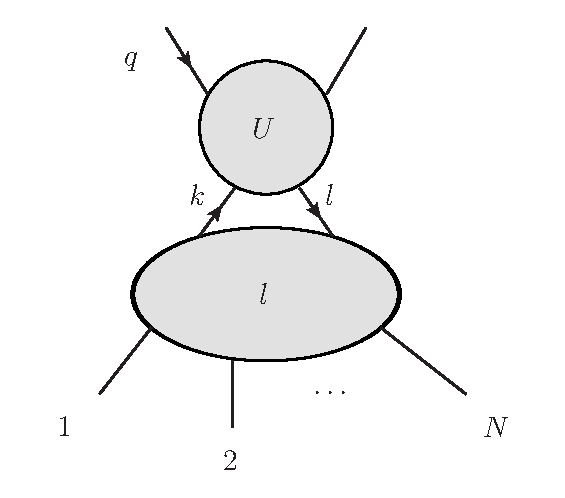
\includegraphics[width=0.35\textwidth]{Graphs/fig1021.eps} 
\caption{}
\label{fig:10.2.1}
\end{figure}

Since the UV subgraph $U$ is, to the leading power of $q^2$, independent of the external momenta $k$ and $l$ flowing into it, we may replace $U$ by its value when $k=l=m=0$, and replace the IR subgraph $I$ by an insertion of a vertex for $\phi^2/2$ in the Green's function. This allows us to factorise the two leg UV subgraph from the rest of the N-point IR diagram. At large $q$, we only need to care about $U$ with the 2 extra external lines. This is why the diagram in Figure \ref{fig:10.1.3abc}(a) is representative and highly relevant to the OPE, as it is itself of the form $U$.

\subsubsection{Constructing Wilson Coefficients}
Now to actually construct the expansion, we have to consider the leading contribution when all the momenta in $U$ is large. In the case where we have large momenta contained within a proper subregion of $U$ (so that there is a further cut within $U$ into $\Hat{U}$ with large momenta and $U/\Hat{U}$ with small momenta), the contribution of U to the Wilson coefficient is defined such that these contributions are subtracted out. We are then ready to use the technique applied to Figure \ref{fig:10.1.3abc} on U, where we evaluated and integrate Figure \ref{fig:10.1.3abc}(c) at $k=l=m=0$ to obtain the leading order contribution to the Wilson coefficient at large $q$. 

\section{Proof} \label{proof}

Now, we will prove the operator product expansion using $\phi^4$-theory as a concrete example. As a reminder, consider the Green's function

\begin{equation}
    G_{N+2}(x, p_1,\dots, p_n) = \mel{0}{T\phi(x)\phi(0)\Tilde{\phi}(p_1)\dots\Tilde{\phi}}{0},
\end{equation}
where each $\phi(x)$ and $\phi(0)$ is connected to some external line. If we rescale $x \rightarrow kx$, for some scale, $k$, we can construct a general decomposition of the form:

\begin{equation}
    G_{N+2}(kx, p_1,\dots, p_n) = C(k^2x^2)\mel{0}{T\frac{1}{2}\phi(0)^2\Tilde{\phi}(p_1)\dots\Tilde{\phi}}{0} + r_{N+2}(kx,p_1,\dots,p_N),
    \label{green's decomposed}
\end{equation}
for some remainder term, $r_{N+2}$.     

We note that, in every order of perturbation theory, the coefficient $C(k^2x^2)$ behaves like $(k^2)^0\log f(k)$ when the scaling parameter $k\rightarrow 0$, while the remainder $r_{N+2}\rightarrow0$ like the power of $k$. On the other hand, if we examine the Green's function in momentum space, we have 

\begin{equation}
    G_{N+2}(kx, p_1,\dots, p_n) = \Tilde{C}(q^2/k^2)\mel{0}{T\frac{1}{2}\phi(0)^2\Tilde{\phi}(p_1)\dots\Tilde{\phi}}{0} + r_{N+2}(q/k,p_1,\dots,p_N).
    \label{green with remainder}
\end{equation}
Now, recall the definition of the Fourier transform

\begin{equation}
    G_{N+2}(kx,p_1,\dots,p_N) = \int \frac{d^4q}{(2\pi)^4} \, e^{-iq\cdot x} \, \Tilde{G}_{N+2}(q/k,p_1,\dots,p_N).
    \label{green with remainder in momentum}
\end{equation}
We find that $\mathrm{dim}\,\Tilde{G} = \mathrm{dim}\,G-4$ and therefore $\mathrm{dim}\,\Tilde{C}(q/k) = \mathrm{dim}\,C(kx)-4$. Since the coefficients in position space are dimensionless, we find that $\mathrm{dim}\,\Tilde{C}(q/k)=-4$. Thus, when we send the scaling parameter $k\rightarrow 0$, or $q/k \rightarrow \infty$, we will find that $\Tilde{C}(q/k)$ behaves like $(k/q)^4 \log f(q/k) $ and the remainder term is smaller by a power of $q/k$. 

\subsection{Construction of the Remainder}\label{construct remainder}

As mentioned before, we will work in $\phi^4$-theory as an example, but this can be generalised with  some effort. In any case, the Lagrangian is the usual

\begin{equation}
    \mathcal{L}= \frac{1}{2}\partial_\mu\phi\partial^\mu\phi - \frac{1}{2}m^2\phi^2 - \frac{g}{4!}\phi^4.
\end{equation}

Let $\Gamma$ represent the Feynman graph we are interested in. The renormalised graph, which we will call $R(\Gamma)$, is $\Gamma$ minus the counterterms which subtract away the UV divergences. Then, $R(\Gamma)$ is a contribution of $\Gamma$ to the Green's function, $G_{N+2}$. Looking back at Equation \ref{green's decomposed}, we still have the remainder term to consider. Let's call it $r(\Gamma)$. This remainder term contains other counterterms that remove not only the UV divergent terms but also the leading $x\rightarrow 0$ or $q \rightarrow \infty$ behaviour of $\Gamma$. In this sense, $R(\Gamma) - r(\Gamma)$ will give us the Wilson coefficient, that is, the first term in Equation \ref{green with remainder} and \ref{green with remainder in momentum}.

To determine the form of $r(\Gamma)$, we take inspiration from looking at how the renormalised graph, $R(\Gamma)$, is constructed. Recall that UV divergences arise from regions with high loop momenta. We employ the following expression to represent the standard programme of renormalisation,

\begin{equation}
    R(\Gamma) = \Gamma - \sum_\gamma C_\gamma(\Gamma),
\end{equation}
where the sum is over all subgraphs, $\gamma$ of $\Gamma$ and $C_\gamma(\Gamma)$ is $\Gamma$ with the subgraph $\gamma$ \textit{replaced by its large-momentum divergence}. We define $C_\gamma(\Gamma)$ to be non-zero only if $\gamma$ is a disjoint union of one or more 1PI diagrams, $\gamma_1,\dots,\gamma_n$\footnote{see example in \S\ref{example3}.}. In this case, each subgraph $\gamma_i$ is replaced by a counterterm vertex $C(\gamma_i)$, which contains the divergent part of $\gamma_i$. We have to make sure no double counting of divergences occur. To that end, we subtract the sub-divergences first:

\begin{equation}
    C(\gamma_i) = \mathcal{P}\left(\gamma_i - \sum_{\delta \varsubsetneq \gamma}C_\delta(\gamma_i)\right).
    \label{counterterm gamma}
\end{equation}
Let's examine this counterterm expression carefully. As in the paragraph above, $C_\delta(\gamma_i)$ tells us to replace the UV divergent subgraph, $\delta$, of our the 1PI graph, $\gamma_i$, with its large momentum divergence, \textit{assuming} that the $\delta$ subgraph is not $\gamma_i$ itself. We have also introduced a new operator, $\mathcal{P}$, which picks out the pole component in $d=4$. This recursion procedure makes sure we do not double count the poles. 

Now that we have an idea of how to isolate counterterms to obtain the renormalised graph, $R(\Gamma)$, we will try a similar strategy for the remainder term, $r(\Gamma)$. First, we remind ourselves that the leading short-distance behaviour, where $x\rightarrow 0$, of $\Gamma$ arises from two momentum regions:

\begin{enumerate}
    \item $q$ finite, and
    \item $q\rightarrow \infty$, where the U region in Figure \ref{fig:10.2.1} receives large momentum contribution.
\end{enumerate}

Now, we define $r(\Gamma)$ to be $\Gamma$ with all the UV divergences \textit{and} with the leading small-$x$ behaviour subtracted, that is

\begin{equation} \label{small_r}
    r(\Gamma) = R(\Gamma) - \sum_\delta \sum_\gamma L_{\gamma \cup \delta}(\Gamma).
\end{equation}
Again, $\delta$ are the subgraphs with UV divergences and the $\gamma$ are the subgraphs of $\Gamma$ such that $\gamma\cap\delta=\varnothing$, \textit{i.e.} the subgraphs that do not intersect with $\delta$. For example, in Figure \ref{fig:10.2.1}, the $\delta$ would be the `U' region and the $\gamma$ would be the bottom subgraph with the $N$ external legs. 

$L_{\gamma\cup\delta}(\Gamma)$ is used to extract the contribution that comes from regions with momenta of $\mathcal{O}(1/x)$ in $\delta$ subgraphs and momenta that go to infinity in $\gamma$ subgraphs. As above, we define the subtraction $L_{\gamma\cup\delta}(\Gamma)$ to be zero unless $\gamma$ is a disjoint union of 1PI, $\gamma_i$. In this case, we can replace each $\gamma_i$ with its counterterm $C(\gamma_i)$ defined in Equation \ref{counterterm gamma}. Additionally, we can replace the $\delta$ graphs by $L(\delta)$. $L(\delta)$ now contains the leading behaviour of internal lines with large momenta. As before, there are subgraphs $\delta'$ that carry momenta of $\mathcal{O}(q)$ and others that carry small momenta. To avoid double counting, we subtract them off in our definition of $L(\delta)$:

\begin{equation} \label{largeQ_recursion}
    L(\delta) = \mathcal{T} \left( \delta - \sum_{\substack{\delta'\varsubsetneq \delta \\ \gamma\cap\delta = \varnothing }} L_{\gamma\cup\delta'}(\delta) \right).
\end{equation}
Let us examine this expression closer:  The $\mathcal{T}$ operator picks out the leading $x\rightarrow 0$ behaviour. Recall from \S\ref{large q}, this behaviour is independent of the mass term, $m$, and the external momenta, $p_i$, for $i=1,\dots N$, so the operator in effect evaluates the parenthesis by setting $m=p_i=0, \forall i$.

In summary, the recipe for obtaining $r(\Gamma)$ from a given graph $\Gamma$ is to:
\begin{enumerate}
    \item Identify a subgraph $\delta$ of $\Gamma$, which looks like $U$ in Figure \ref{fig:10.2.1}, i.e. containing the two open upper legs and two lower legs.
    \item For such $\delta$, identify all subgraphs $\gamma$ which do not intersect $\delta$.
    \item For this pair of $\delta$ and $\gamma$, 
    \begin{enumerate}
        \item replace $\gamma$ with its counterterm $C(\gamma)$ using Equation \ref{counterterm gamma} to take care of divergences within $\gamma$ without double counting ) and
        \item replace $\delta$ with its leading $x \rightarrow 0$/$q \rightarrow \infty$ behaviour graph, $L(\delta)$. This is done using the $\mathcal{T}$ operator in Equation \ref{largeQ_recursion}).
    \end{enumerate}
    \item Sum over all $\delta$'s and their corresponding $\gamma$ using the Equation \ref{small_r}, $r(\Gamma) = R(\Gamma) - \sum_\delta \sum_\gamma L_{\gamma \cup \delta}(\Gamma)$
\end{enumerate}


Now that we have a definition for $R(\Gamma)$ and $r(\Gamma)$, it's time to apply them to some examples.\\ \\

\noindent\textbf{Example 1: Figure 10.1.1}\\

\begin{figure}[H]
\centering
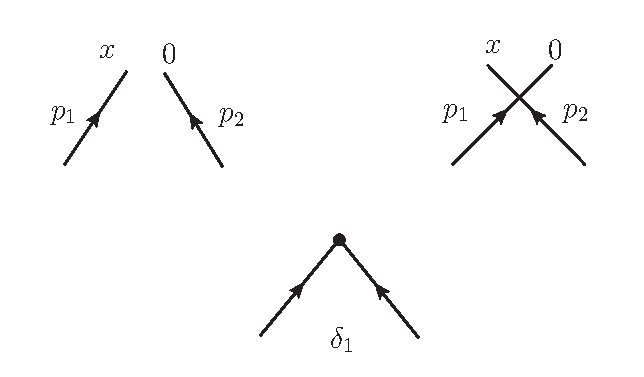
\includegraphics[width=0.35\textwidth]{Graphs/Fig1011.eps} 
\caption{}
\label{fig:example1}
\end{figure}
Let us consider the simplest example: tree level contribution to $\mel{0}{T\phi(x)\phi(0)\Tilde{\phi}(p_1)\Tilde{\phi}(p_2)}{0}$, which corresponds to Figure \ref{fig:example1}. The only $\delta$ graph one can construct is with $\phi(x)\phi(0)$ only, \textit{i.e.} no $\phi^4$ insertion. This is exactly that of Figure \ref{fig:10.2.1}, but with the `U' region replaced trivially by just the legs of the propagators. One can also make a trivial check that Figure \ref{fig:example1} has no subgraphs. In any case, let's call it $\delta_1$. Now, we have

\begin{equation}
\begin{split}
    L(\delta_1) &= \mathcal{T}\left( \delta_1 - \sum_{\substack{\delta'\varsubsetneq \delta_1 \\ \gamma\cap\delta_1 = \varnothing }} L_{\gamma\cup\delta'}(\delta_1)  \right),\\
    &= \mathcal{T}(\delta_1) = \delta_1\vert_{m=p_i=0},\\
    &= (e^{-ip_1\cdot x} + e^{-ip_2\cdot x})\vert_{m=p_i=0},\\
    L(\delta_1) &=2,
\end{split}
\label{delta1}
\end{equation}
where we note that the $L_{\gamma\cup\delta'}(\delta_1)$ term vanishes trivially since $\delta_1$ has no subgraphs $\gamma$.  If we compare the results of Equation \ref{delta1} with that of Equation \ref{small x expansion}, we find that $L(\delta_1)$ is exactly the zeroth order term in the Wilson expansion, up to factors of external propagators. If we call Figure \ref{fig:example1} $\Gamma_1$, then the remainder term is 

\begin{equation}
    r(\Gamma_1) = \Gamma_1 - L(\delta_1).
    \label{rGamma1}
\end{equation}
Given the definition of the remainder term, and that Figure \ref{fig:example1} is only a tree-level graph, it is clear in hindsight that the remainder is exactly the original graph minus its Wilson expansion.\\

\noindent\textbf{Example 2: Figure 10.1.3}

\begin{figure}[h!]
\centering
\begin{subfigure}
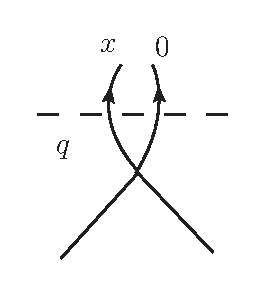
\includegraphics[scale=0.65]{Graphs/Fig1013.eps} 
\label{fig:10.1.3}
\caption{An $\mathcal{O}(g)$ graph. The dashed line indicates where the subgraphs $\delta_1$(above), $\gamma_1$(below) and $\delta_2$ (whole) are.}
\end{subfigure}

\begin{subfigure}
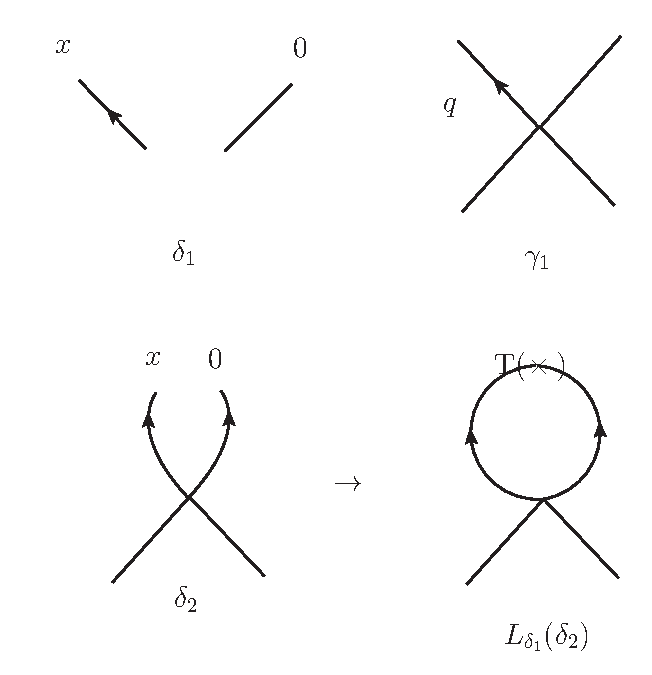
\includegraphics[scale=0.65]{Graphs/Fig1013delta.eps} 
\label{fig:10.1.3delta}
\caption{Possible subgraphs from an $\mathcal{O}(g)$ graph.}
\end{subfigure}
\end{figure}
Now we consider the $\mathcal{O}(g)$ term in $\mel{0}{T\phi(x)\phi(0)\Tilde{\phi}(p_1)\Tilde{\phi}(p_2)}{0}$. Let's call it $\Gamma_2$. First, note that $\delta_1$ from before is embedded as a subgraph in $\Gamma_2$ (above the dashed line); it also has another subgraph of the form $U$. This contains the `loop' and the two lower legs \textit{i.e.} the whole graph. We will label as $\delta_2$. 

Let us first deal with the terms in $\sum_{\delta,\gamma} L_{\gamma \cup \delta}(\Gamma_2)$ that involves $\delta_1$. There are two such terms:
\begin{enumerate}
    \item $L_{\gamma_1 \cup \delta_1}(\Gamma_2)$ and
    \item $L_{\delta_1}(\Gamma_2)$, i.e. $\gamma = \varnothing$.
\end{enumerate}
In the first case, since $\gamma_1$ is finite, its counterterm vertex is 0, and replacing it with its counterterm will yield zero; i.e.
\begin{equation}
    L_{\gamma_1 \cup \delta_1}(\Gamma_2) = 0
\end{equation}

As for the second case,$\gamma$ is empty, so all we have to do is to replace $\delta_1$ with $L(\delta_1)$.  Essentially, we have just replaced the top open vertex with a closed vertex by setting the momentum flowing through it to 0 (see Figure \ref{fig:10.1.3delta}). This graph evaluates to:
\begin{equation}
    L_{\delta_1}(\Gamma_2) = i\mu^{4-d}g\int \frac{d^dq}{(2\pi)^d}\frac{1}{(q^2-m^2)((p_1+p_2-q)^2-m^2)}
\end{equation}
and the constant numerator is from the closed vertex.

Next, we look at the contribution from $\delta_2$. Note that $\delta_1$ is a subgraph of $\delta_2$, so we have to apply the procedure in Equation \ref{largeQ_recursion} to obtain $L(\delta_2)$. This makes it a more interesting case than Figure \ref{fig:example1}. We have

\begin{equation}
    \begin{split}
        L(\delta_2) &= (\delta_2 - L_{\delta_1}(\delta_2))\vert_{m=p_1=p_2=0},\\
        &=i\mu^{4-d}g \int \frac{d^dq}{(2\pi)^d} \frac{e^{-iq\cdot x}-1}{(q^2-m^2)((p_1+p_2-q)^2-m^2)}\bigg\vert_{m=p_1=p_2=0},\\
        &=i\mu^{4-d}g \int \frac{d^dq}{(2\pi)^d} \frac{e^{-iq\cdot x}-1}{(q^2)^2}.
    \end{split}
\end{equation}
In this example, we see that $L_{\delta_1}(\delta_2)$ in effect tells us to replace the UV divergent region in $\delta_2$ with $L(\delta_1)$, where we can expect $x\rightarrow 0$. Since $\delta_2$ is the entirety of $\Gamma_2$, there are no further subgraphs $\gamma$ which we need to consider. Furthermore, we can also see that $L_{\delta_2}(\Gamma_2)=L(\delta_2)$, since the LHS involves replacing the entire graph with $L(\delta_2)$.



Putting all of these together, our remainder term for $\Gamma_2$ becomes

\begin{equation}
    \begin{split}
        r(\Gamma_2) &= R(\Gamma_2) - \sum_{\delta,\gamma} L_{\gamma \cup \delta}(\Gamma_2),\\
        &= R(\Gamma_2) - L_{\delta_1}(\Gamma_2) - L_{\delta_2}(\Gamma_2),\\
        &=i\mu^{4-d}g \int \frac{d^dq}{(2\pi)^d} \frac{e^{-iq\cdot x}}{(q^2-m^2)((p_1+p_2-q)^2-m^2)} \\
        &\quad\quad\quad\quad\quad\quad\quad\quad\quad - \frac{1}{(q^2-m^2)((p_1+p_2-q)^2-m^2)} - \frac{e^{-iq\cdot x}-1}{(q^2)^2},
    \end{split}
\end{equation}
where in the final line, we identify the first term as the term to be renormalised ($R(\Gamma_2)$) and the second and  third term belonging to $L_{\delta_1}(\Gamma_2)$ and $L_{\delta_2}(\Gamma_2)$ respectively. \\

\noindent\textbf{Example 3: An $\mathcal{O}(g^2)$ graph.}\label{example3}

Finally, let us apply the method on a less trivial example. Consider the $\mathcal{O}(g^2)$ terms which contribute to $\mel{0}{T\phi(x)\phi(0)\Tilde{\phi}(p_1)\Tilde{\phi}(p_2)}{0}$. We will proceed systematically, using the prescription in  \S\ref{construct remainder} to obtain the expansion. An example graph that contributes to the expansion is $\Gamma_3$ below:
\begin{figure}[H]
\centering
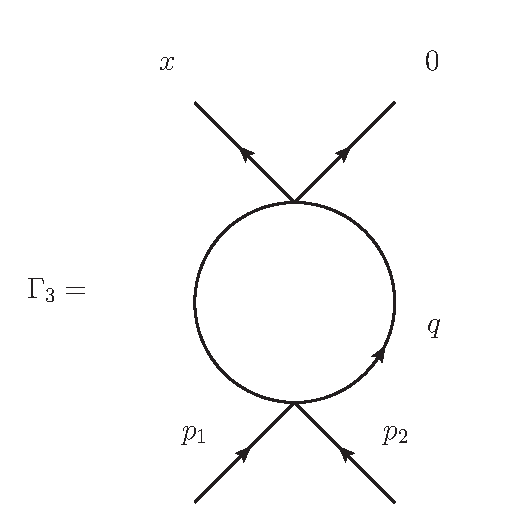
\includegraphics[width=0.35\textwidth]{Graphs/Gamma.eps}
\end{figure}\\

The graph itself evaluates to (ignore factors of i and minus signs)
\begin{equation} \label{Gamma_3}
    \Gamma = \frac{1}{p_1^2-m^2}\frac{g^2}{p_2^2-m^2} \int \frac{d^dk}{(2\pi)^d}\frac{1}{(k^2-m^2)[(k+p_1+p_2)^2-m^2]}\int \frac{d^dq}{(2\pi)^d}\frac{e^{-iq\cdot x}}{(q^2-m^2)(q_2^2-m^2)}.
\end{equation}






From this diagram $\Gamma_3$, there are 3 possible $\delta_i$'s. Note that the $\delta_1$ and $\delta_2$ in Figure \ref{gamma3&delta} are identical to the ones considered in the previous examples. $\delta_3$ on the other hand is the entire graph itself. Thus, we have:\\
\begin{figure}[H]
\centering
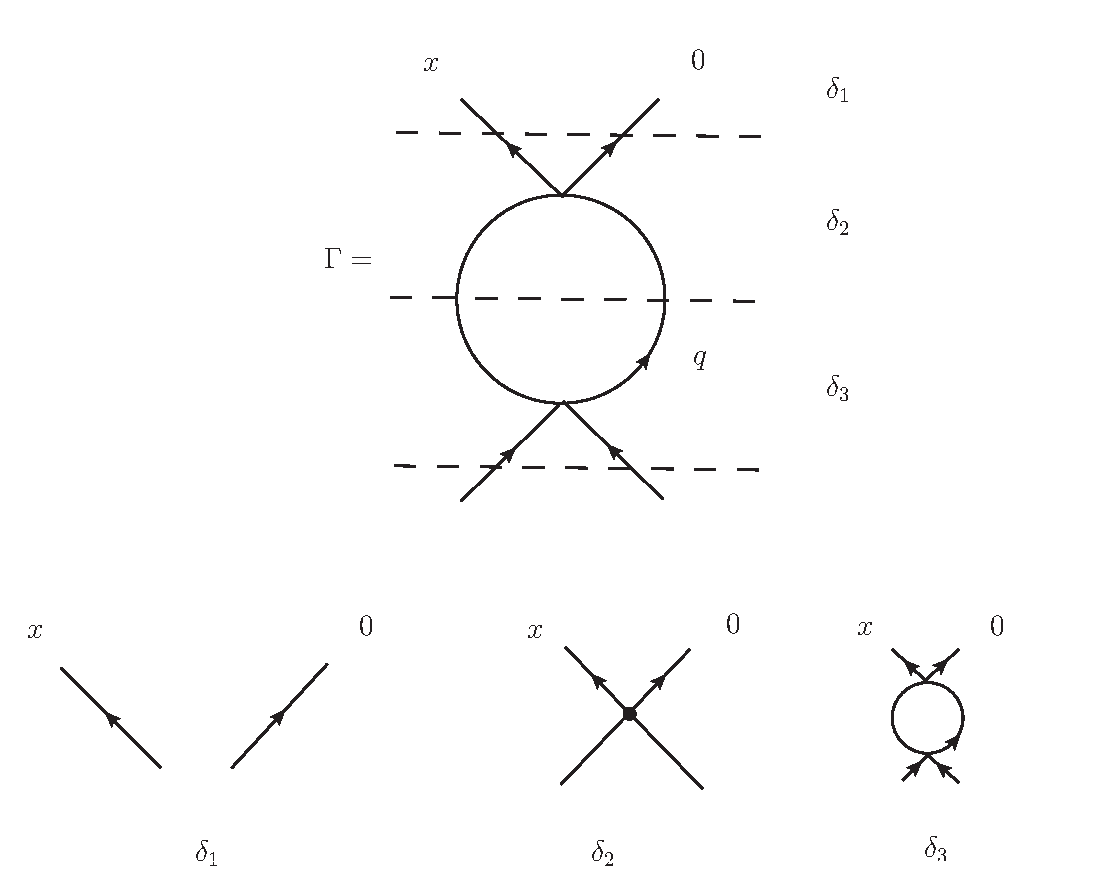
\includegraphics[width=0.5\textwidth]{Graphs/Gammadelta.eps}
\label{gamma3&delta}
\end{figure}\\
Let us first consider the terms contributing from $\delta_1$, \textit{i.e.} $\sum_{\gamma}L_{\gamma \cup \delta_1}(\Gamma_3)$. There are three possible terms:
\begin{enumerate}
    \item $L_{\delta_1}(\Gamma_3)$,
    \item $L_{\gamma_1 \cup \delta_1}(\Gamma_3)$ and
    \item $L_{\gamma_2 \cup \delta_1}(\Gamma_3)$.
\end{enumerate}
where $\gamma_1$ and $\gamma_2$ are defined from 
\begin{figure}[H]
\centering
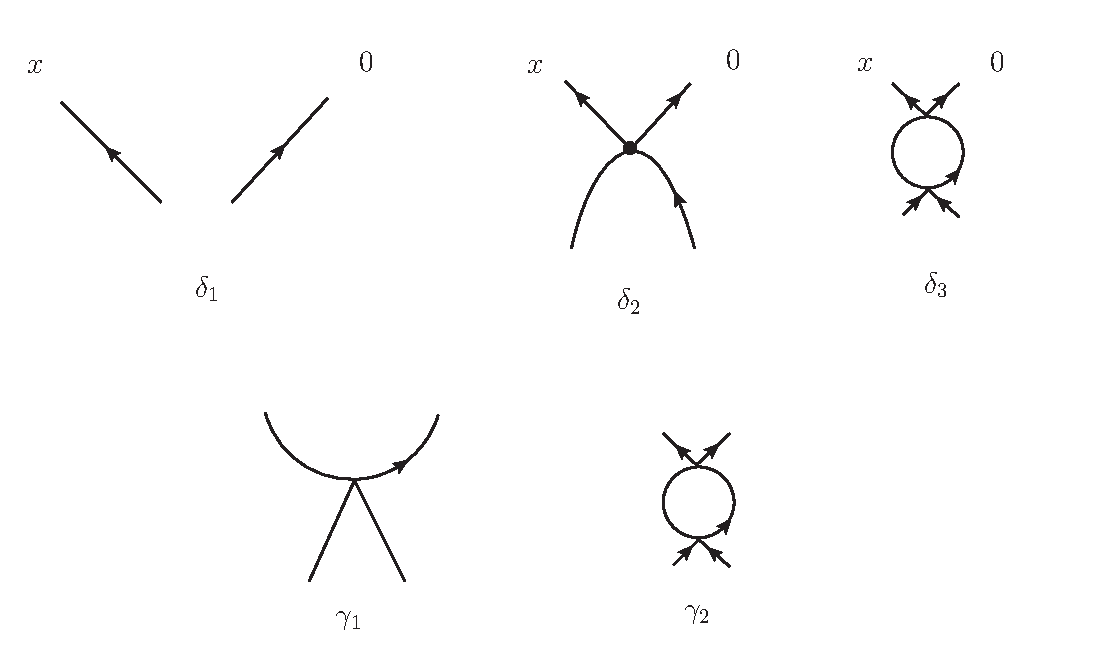
\includegraphics[width=0.75\textwidth]{Graphs/deltagamma.eps}
\end{figure}\\
They are found in the lower parts of the graph $\Gamma_3$. Let us compute the contributions from each term.

Firstly, $L_{\delta_1}$ (we omit the ($\Gamma_3$) from this point onwards; it is implied) is obtained simply by replacing $\delta_1$ by $L(\delta_1)$, i.e. closing the top and setting $q=0$ for the numerator. We then have
\begin{equation}
    \text{I}:=L_{\delta_1} = ... \int \frac{d^dk}{(2\pi)^d}\frac{1}{(k^2-m^2)[(k+p_1+p_2)^2-m^2]}\int \frac{d^dq}{(2\pi)^d}\frac{1}{(q^2-m^2)(q_2^2-m^2)}.
\end{equation}
where $...$ are the prefactors before the first integral in equation \ref{Gamma_3}.

Next, as we have seen before, since $\gamma_1$ is finite, its counter-term is 0. Therefore the term 
\begin{equation}
    L_{\gamma_1 \cup \delta_1} = 0
\end{equation}

Next, we evaluate the last term contributing to $\delta_1$: $L_{\gamma_2 \cup \delta_1}$. In this term, $\gamma_2$ is divergent, therefore we need to replace it with its counterterm; this is illustrated in Figure \ref{fig:Ldelta} below: 
\begin{figure}[H]
\centering
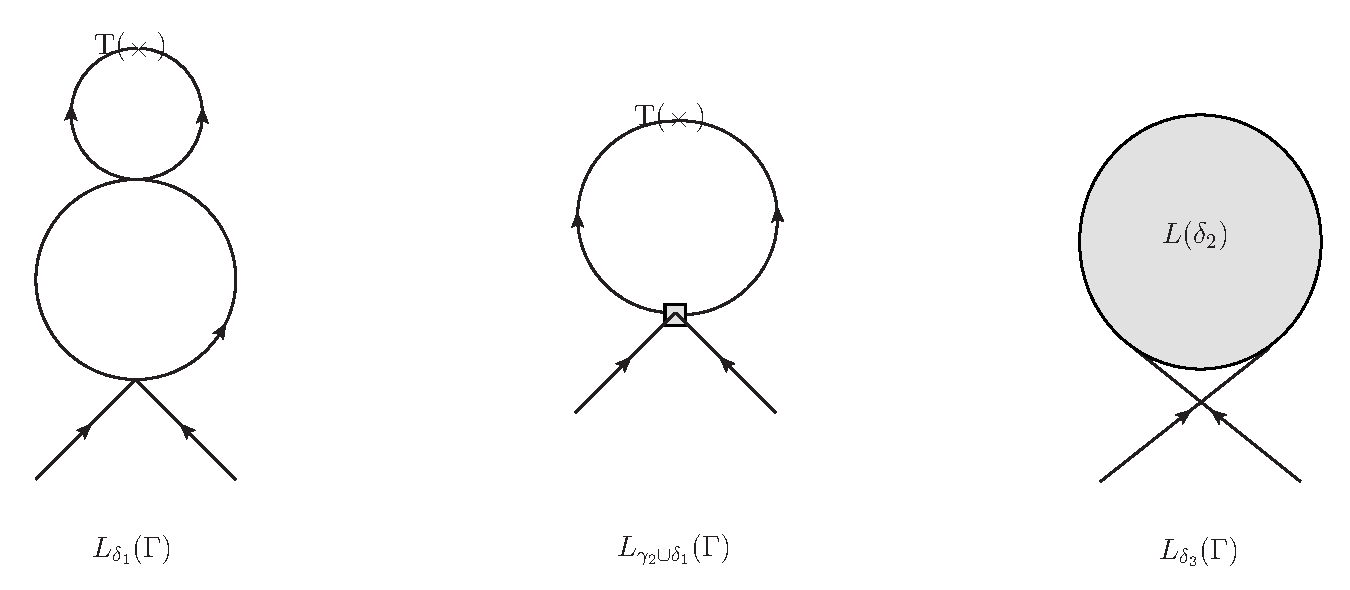
\includegraphics[width=0.75\textwidth]{Graphs/LGammadelta.eps}
\label{fig:Ldelta}
\caption{}
\end{figure}\\
where the box represents the 1-loop counterterm for the 4-leg vertex. The diagram therefore evaluates to
\begin{equation}
    \text{II}:=L_{\gamma_2 \cup \delta_1}=...\times \mathcal{P}\qty(\int\frac{d^dk}{(2\pi)^d}\frac{1}{(k^2-m^2)[(k+p_1+p_2)^2-m^2]})\int \frac{d^dq}{(2\pi)^d}\frac{1}{(q^2-m^2)(q_2^2-m^2)}.
\end{equation}
In MS scheme, (Peskin p.327 \cite{Peskin:1995ev})
\begin{equation}
    \mathcal{P}\qty(\int\frac{d^dk}{(2\pi)^d}\frac{1}{(k^2-m^2)[(k+p_1+p_2)^2-m^2]}) \xrightarrow{\text{d\rightarrow4}} \frac{1}{8\pi^2 \epsilon}.
\end{equation}
In other schemes, this term will look slightly different.

Next, let us consider the terms contributing from $\delta_2$, i.e. $\sum_{\gamma}L_{\gamma \cup \delta_2}(\Gamma_3)$. There are two possible terms:
\begin{enumerate}
    \item $L_{\delta_2}$
    \item $L_{\gamma_1 \cup \delta_2}$
\end{enumerate}
Consider first the term $L_{\delta_2}$. It is obtained by replacing $\delta_2$ with $L(\delta_2)$, and is drawn in the diagram above. We have in fact already calculated $L(\delta_2)$ from the previous example, so we can easily evaluate this diagram:
\begin{equation}
    \text{III}:=L_{\delta_2}(\Gamma_3)= ...\int\frac{d^dk}{(2\pi)^d}\frac{1}{(k^2-m^2)[(k+p_1+p_2)^2-m^2]}\int\frac{d^dq}{(2\pi)^d}\frac{e^{-iq\cdot x}-1}{(q^2)^2}.
\end{equation}
And we note that again, since $\gamma_1$ is finite, 
\begin{equation}
    L_{\gamma_1 \cup \delta_2} = 0
\end{equation}

Next, we evaluate the terms contributing from $\delta_3$, \textit{i.e.} $\sum_{\gamma}L_{\gamma \cup \delta_3}(\Gamma_3)$. There is only one term, and it is $L_{\delta_3}(\Gamma) = L(\delta_3)$. Using Equation \ref{largeQ_recursion},
\begin{equation}
\begin{split}
    \text{IV}:=L(\delta_3) &= \mathcal{T}(\delta_3-L_{\delta_1}(\delta_3)-L_{\gamma_2 \cup \delta_1}(\delta_3)-L_{\delta_2}(\delta_3)),\\
    &=\mathcal{T}(\delta_3-\text{I}-\text{II}-\text{III}),\\
    &=...(\int\frac{d^dk}{(2\pi)^d}\frac{1}{(k^2)^2}\int\frac{d^dq}{(2\pi)^d}\frac{e^{-iq\cdot x}}{(q^2)^2} - \int\frac{d^dk}{(2\pi)^d}\frac{1}{(k^2)^2}\int\frac{d^dq}{(2\pi)^d}\frac{1}{(q^2)^2}, \\
    &- \frac{1}{8\pi^2 \epsilon}\int\frac{d^dq}{(2\pi)^d}\frac{1}{(q^2)^2}-\int\frac{d^dk}{(2\pi)^d}\frac{1}{(k^2)^2}\int\frac{d^dq}{(2\pi)^d}\frac{e^{-iq\cdot x}-1}{(q^2)^2}),\\
    &= ...\frac{-1}{8\pi^2 \epsilon}\int\frac{d^dq}{(2\pi)^d}\frac{1}{(q^2)^2}.
\end{split}
\end{equation}

We can finally write down the expression for the remainder:
\begin{equation}
\begin{split}
r(\Gamma_3) &= R(\Gamma_3) - \sum_\delta \sum_\gamma L_{\gamma \cup \delta} (\Gamma_3)\\
&=R(\Gamma_3) - \text{I} - \text{II} - \text{III} - \text{IV}.
\end{split}
\end{equation}

The Wilson coefficient contribution of the diagram is then precisely (this will examined in more detail in the next section):
\begin{equation}
    W(\Gamma_3) = \sum_\delta \sum_\gamma L_{\gamma \cup \delta} (\Gamma_3) = \text{I} + \text{II} + \text{III} + \text{IV}.
\end{equation}

The other $\mathcal{O}(g^2)$ term can be constructed similarly using the procedure listed above.

\subsubsection{Recap}
What we have essentially done here is we obtained a general procedure to obtain $R(\Gamma) - r(\Gamma) = \sum_\delta \sum_\gamma L_{\gamma \cup \delta}(\Gamma)$; through this procedure we are left with an expansion in subgraphs that is UV and IR finite (this is explained quite well in Collins \S 10.3.2). This expression contains the leading $x \rightarrow 0$ behaviour of $R(\Gamma)$, and is all-important for obtaining the Wilson expansion. The next step is then to show that the sum of this expansion in subgraphs will give us the Wilson coefficient.

\subsection{Obtaining Wilson Coefficients}
Let us remind ourselves again what we are trying to obtain here: we wish to obtain the $C_{\phi^2}(x)$ term in equation \ref{small x ope}, as explained at the end of section \S\ref{10.1.1}. From the above discussion, we know that each diagram $\Gamma$ will have many subgraphs $\delta$'s which contribute to $C_{\phi^2}(x)$, and we need to sum over these contribution to obtain the full $C_{\phi^2}(x)$. More concretely, for a specific diagram $\Gamma$, \textit{if} $W(\Gamma)$ (which contains the leading $x \rightarrow 0$ behaviour of $R(\Gamma)$) could be put in the form of the final line:
\begin{equation}
\begin{split}
\label{wilson_coeff_1}
    W(\Gamma) &\equiv R(\Gamma) - r(\Gamma)\\ 
    &= \sum_\delta \bar{C}(\delta) R(\Gamma/\delta)
\end{split}
\end{equation}
where $\Gamma/\delta$ is $\Gamma$ contracted to a point, i.e., replaced by a $\phi^2$ vertex, \textit{then} the contribution to the Wilson coefficient $C_{\phi^2}(x)$ from the particular graph is
\begin{equation}
    C_{\phi^2}(x) = \sum_\delta \bar{C}(\delta)
\end{equation}
This can be seen because when we sum over the $\Gamma$ in equation \ref{wilson_coeff_1}, this is equivalent to summing over $\delta$ and $\Gamma/\delta$ independently.

In the previous section, we have obtained an expression for $W(\Gamma)$:
\begin{equation}
    W(\Gamma) = \sum_\delta L_\delta\qty(\sum_{\substack{\gamma \\ \gamma \cap \delta \neq \varnothing}}C_\gamma (\Gamma))
\end{equation}
and we need to massage it into the form in equation \ref{wilson_coeff_1}. The crucial point to note now is that for a general graph $\Gamma$ and its subgraphs $\delta$, we do not necessarily know what $\bar{C}(\delta)$ is, nor do we know that it can be converted into the form of equation \ref{wilson_coeff_1}. However, we do know what $\bar{C}(\delta)$ is for the smallest, lowest-order subgraph. From the discussion in \S\ref{10.1.1} and our example 1 in the previous section, the following subgraph
\begin{figure}[H]
\centering
\includegraphics*[width=0.5\textwidth]{Graphs/Fig1011a.eps}
\caption{Lowest order subgraph}
\end{figure}\\
gives $W(\Gamma_1) = R(\Gamma_1)-r(\Gamma_1) = L(\delta_1) = 2$ (see equation \ref{rGamma1}); and from the taylor expansion discussion in \S\ref{10.1.1}, we know that $\bar{C}(\Gamma_1)=1$. Equipped with this, we can now \textit{define} for an arbitrary graph $U$:
\begin{equation}
    2\bar{C}(U) = W(U) - \sum_{\delta \varsubsetneq U}\bar{C}(\delta)R(U/\delta)
\label{CbarU}
\end{equation}
with the factor of 2 accounting for the lowest-order operator as mentioned. This equation gives a recursive definition to build up $\bar{C}(U)$ for larger subgraphs, up to the biggest subgraph $U = \Gamma$. What remains to be shown is that this definition can in fact consistently allow us to massage $W(\Gamma)$ into the desired form. 

Let us now choose $U$ to be the biggest possible subgraph of $\Gamma$ that is in the form of figure \ref{fig:10.2.1} (which by Weinberg's theorem are the only important ones). In this case, all subgraphs $\delta$ are contained in $U$, and so $W(\Gamma)$ are separable into its $U$ and $I$:
\begin{equation}
\begin{split}
    W(\Gamma) &= \int \frac{d^4k d^4l}{(2\pi)^8}W(U)R(I)\\
    &\equiv W(U) \otimes R(I)
\end{split}
\end{equation}
since no divergent 1PI subgraphs include parts of both $U$ and $I$. Now, because of how $\bar{C}(U)$ is defined in equation \ref{CbarU}, $W(U)$ can in fact be decomposed into the form in equation \ref{wilson_coeff_1}. Then, 
\begin{equation}
\begin{split}
    W(\Gamma) &= \sum_\delta \bar{C}(\delta) R(U/\delta) \otimes R(I)\\
    &=\sum_\delta \bar{C}(\delta) R(\Gamma/\delta)
\end{split}
\end{equation}
The last step is possible since
\begin{enumerate}
    \item the graphs for $\Gamma/\delta$ are of the form $U/\delta$ times $I$, and
    \item UV divergent 1PI subgraphs are entirely within $U/\delta$ or within $I$. 
\end{enumerate}
It is important to realise that it is because of the use of power-counting arguments, that we can restrict ultra-violet divergences to within $U/\delta$. 


\subsection{Conclusion}
And there we have it: a systematic procedure for obtaining the wilson coefficients $C_{\phi^2}(x)$ in equation \ref{small x ope}. This can easily be generalised to obtain the Wilson coefficients for other operators. These can be shown to be independent of $m, k, l$, and is a purely ultra-violet object, as Collins shows in \S 10.3.3. 



\bibliographystyle{ieeetr} 
\bibliography{opeBib.bib}

\end{document}
